\documentclass[11pt]{article}
\usepackage[a4paper,margin=24mm]{geometry}
\usepackage{amsmath,amssymb,booktabs,graphicx,microtype}
\usepackage[hidelinks]{hyperref}
\usepackage{siunitx}
\usepackage{xcolor}
\graphicspath{{../figures/}}
\setlength{\parindent}{0pt}
\setlength{\parskip}{0.65em}
\title{A Computational-Basis Metric Blind Spot\\under Phase-Flip Noise}
\author{Q-Reliability Lab}
\date{22 October 2026}

\begin{document}
\maketitle

\begin{abstract}
This study asks whether the computational-basis success probability
$P(00)+P(11)$ can incorrectly certify a noisy Bell-state circuit.  Starting
from $|\Phi^+\rangle=(|00\rangle+|11\rangle)/\sqrt{2}$, we apply a phase-flip
channel with probability $p$ to the first qubit and evaluate 101 deterministic
density-matrix simulations for $p=0,0.01,\ldots,1$.  The measured success
probability is exactly $1$ throughout the sweep, whereas fidelity to
$|\Phi^+\rangle$ falls from $1$ to $0$ and
$\operatorname{Re}(\rho_{00,11})$ changes from $0.5$ to $-0.5$.  At $p=0.5$
the off-diagonal coherence vanishes even though the success metric remains
perfect.  Thus the selected task metric is blind to this phase error.  This is
an analytic, noiseless classical simulation of a simplified channel, not a
measurement of a physical device or a complete CNOT characterization.
\end{abstract}

\section{Introduction}
Near-term quantum circuits are limited by imperfect gates, decoherence, and
measurement noise, so a useful benchmark must state what its metric can and
cannot observe \cite{preskill2018nisq}.  A task success probability is defined
by a chosen set of acceptable classical outputs.  State fidelity instead asks
how close the complete output state is to a target state
\cite{nielsenchuang2010}.  These questions coincide only in special cases.

For a Bell-state preparation task, it is tempting to call both $00$ and $11$
successful and report $P(00)+P(11)$.  That metric reads diagonal density-matrix
elements, but the relative phase distinguishing $|\Phi^+\rangle$ from
$|\Phi^-\rangle$ is encoded off the diagonal.  The present study isolates this
blind spot with a phase-flip channel represented by Kraus operators, a standard
description of open-system evolution \cite{wood2015tensor}.

\section{Methodology}
\subsection{Bell-state preparation}
Order the computational basis as
$(|00\rangle,|01\rangle,|10\rangle,|11\rangle)$.  Beginning with $|00\rangle$,
apply $H$ to the first qubit:
\begin{align}
(H\otimes I)|00\rangle
&=H|0\rangle\otimes I|0\rangle \\
&=\frac{|0\rangle+|1\rangle}{\sqrt{2}}\otimes|0\rangle \\
&=\frac{|00\rangle+|10\rangle}{\sqrt{2}}.
\end{align}
A CNOT with the first qubit as control maps $|00\rangle\mapsto|00\rangle$ and
$|10\rangle\mapsto|11\rangle$, giving
\begin{equation}
|\Phi^+\rangle=\frac{|00\rangle+|11\rangle}{\sqrt{2}}
=\frac{1}{\sqrt{2}}\begin{pmatrix}1&0&0&1\end{pmatrix}^{\!T}.
\end{equation}

The density operator is the outer product
\begin{align}
\rho_+&=|\Phi^+\rangle\langle\Phi^+| \\
&=\frac12(|00\rangle+|11\rangle)(\langle00|+\langle11|)\\
&=\frac12\bigl(|00\rangle\langle00|+|00\rangle\langle11|
  +|11\rangle\langle00|+|11\rangle\langle11|\bigr)\\
&=\frac12\begin{pmatrix}
1&0&0&1\\0&0&0&0\\0&0&0&0\\1&0&0&1
\end{pmatrix}.
\end{align}
Hence $\rho_{00,00}=\rho_{11,11}=1/2$ and the coherence elements are
$\rho_{00,11}=\rho_{11,00}=1/2$.

\subsection{Phase-flip channel and completeness}
On the first qubit, define
\begin{equation}
Z_1=Z\otimes I=\operatorname{diag}(1,1,-1,-1).
\end{equation}
The channel
\begin{equation}
\mathcal{E}_p(\rho)=(1-p)\rho+pZ_1\rho Z_1
\end{equation}
has two Kraus operators
\begin{equation}
E_0=\sqrt{1-p}\,I_4,
\qquad E_1=\sqrt{p}\,Z_1.
\end{equation}
Their completeness relation is explicit:
\begin{align}
E_0^\dagger E_0+E_1^\dagger E_1
&=(1-p)I_4^\dagger I_4+pZ_1^\dagger Z_1\\
&=(1-p)I_4+pZ_1^2\\
&=(1-p)I_4+pI_4=I_4.
\end{align}
Thus the operator-sum map is trace preserving; its Kraus form also guarantees
complete positivity.

Because
\begin{equation}
Z_1|\Phi^+\rangle
=\frac{Z|0\rangle\otimes|0\rangle+Z|1\rangle\otimes|1\rangle}{\sqrt2}
=\frac{|00\rangle-|11\rangle}{\sqrt2}=|\Phi^-\rangle,
\end{equation}
the output is
\begin{equation}
\rho(p)=(1-p)|\Phi^+\rangle\langle\Phi^+|
+p|\Phi^-\rangle\langle\Phi^-|.
\end{equation}
Expanding both projectors gives
\begin{equation}
\rho(p)=\frac12\begin{pmatrix}
1&0&0&1-2p\\
0&0&0&0\\
0&0&0&0\\
1-2p&0&0&1
\end{pmatrix}.
\end{equation}
The index-level transformation follows from
$(Z_1\rho Z_1)_{ij}=z_i z_j\rho_{ij}$, with
$(z_{00},z_{01},z_{10},z_{11})=(1,1,-1,-1)$.  Therefore
\begin{align}
\rho_{00,00}(p)&=(1-p)\frac12+p(1)(1)\frac12=\frac12,\\
\rho_{11,11}(p)&=(1-p)\frac12+p(-1)(-1)\frac12=\frac12,\\
\rho_{00,11}(p)&=(1-p)\frac12+p(1)(-1)\frac12=\frac{1-2p}{2},\\
\rho_{11,00}(p)&=\frac{1-2p}{2}.
\end{align}

\subsection{Metrics}
The computational-basis success probability reads only the populations:
\begin{equation}
S(p)=P(00)+P(11)=\rho_{00,00}(p)+\rho_{11,11}(p)=1.
\end{equation}
Because the target is pure, fidelity reduces to
\begin{align}
F(p)&=\langle\Phi^+|\rho(p)|\Phi^+\rangle\\
&=(1-p)|\langle\Phi^+|\Phi^+\rangle|^2
+p|\langle\Phi^+|\Phi^-\rangle|^2\\
&=(1-p)(1)+p(0)=1-p.
\end{align}
Finally,
\begin{equation}
\operatorname{Re}(\rho_{00,11})=\frac{1-2p}{2},
\qquad |\rho_{00,11}|=\frac{|1-2p|}{2}.
\end{equation}
The signed real part records the phase reversal; magnitude alone does not.

\section{Experiment Setup}
The implementation uses Python, NumPy, and Matplotlib, with pytest for
verification.  It evaluates the exact density matrix for
$p=0,0.01,\ldots,1$, writes 101 rows to a CSV file, and renders two figures.
No random sampling or quantum SDK is used.  From the repository root, run:
\begin{verbatim}
python -m src.phase_error_blind_spot \
  --output experiments/phase_error_sweep.csv --figures figures
\end{verbatim}
The test suite checks Kraus completeness, unit trace, Hermiticity, positive
semidefiniteness with a numerical eigenvalue tolerance, analytic endpoints,
and the stated metric blind spot.

\section{Results}
Table~\ref{tab:results} reports representative rows of the deterministic
101-point sweep.  Values agree with the analytic expressions to floating-point
precision.
\begin{table}[ht]
\centering
\caption{Representative simulated values.  The task metric remains perfect
while fidelity and signed coherence expose the phase error.}
\label{tab:results}
\begin{tabular}{@{}S[table-format=1.2]S[table-format=1.1]S[table-format=1.2]S[table-format=-1.2]S[table-format=1.2]@{}}
\toprule
{$p$} & {$S(p)$} & {$F(p)$} & {$\operatorname{Re}(\rho_{00,11})$} & {$|\rho_{00,11}|$}\\
\midrule
0.00 & 1.0 & 1.00 &  0.50 & 0.50\\
0.25 & 1.0 & 0.75 &  0.25 & 0.25\\
0.50 & 1.0 & 0.50 &  0.00 & 0.00\\
0.75 & 1.0 & 0.25 & -0.25 & 0.25\\
1.00 & 1.0 & 0.00 & -0.50 & 0.50\\
\bottomrule
\end{tabular}
\end{table}

\begin{figure}[ht]
\centering
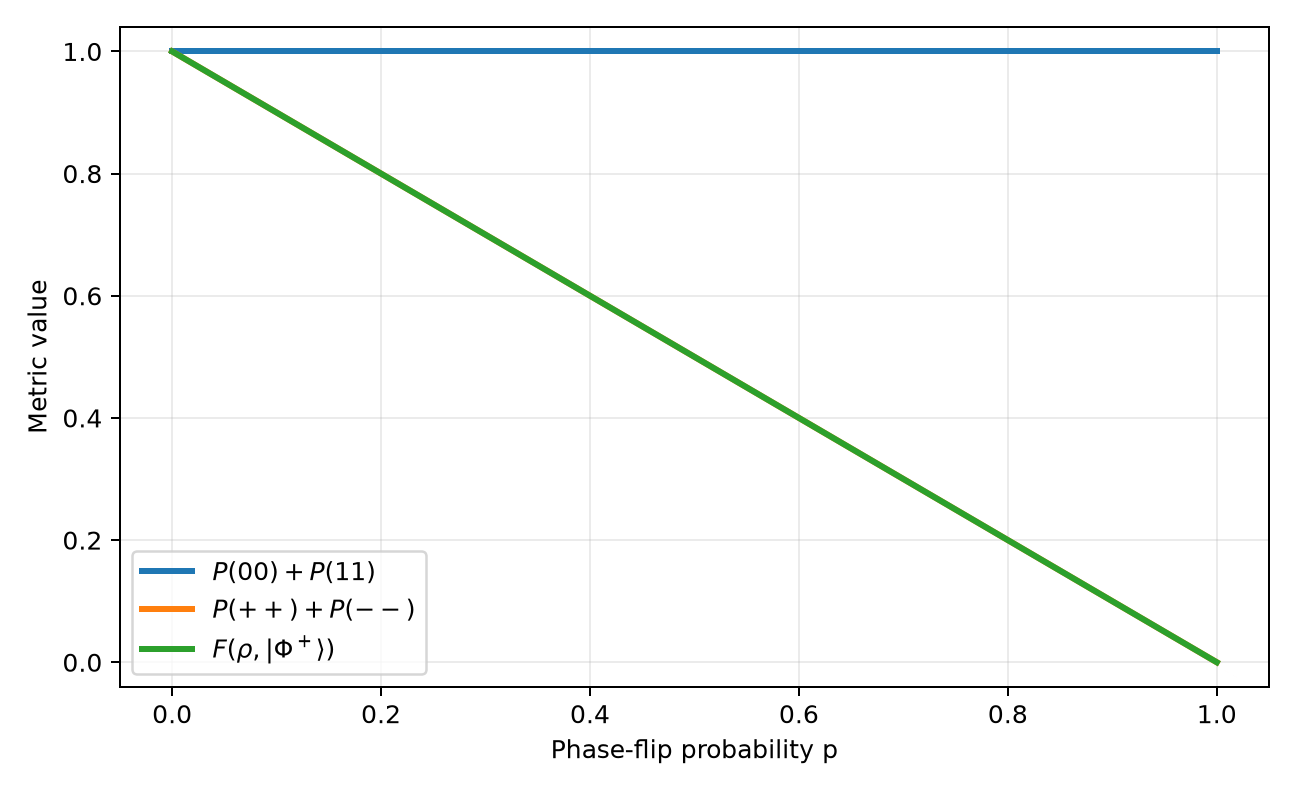
\includegraphics[width=0.86\linewidth]{success_vs_fidelity.png}
\caption{Computational-basis success remains one for every phase-flip
probability, while fidelity falls linearly from one to zero.  The chosen task
metric therefore cannot certify the intended Bell state.}
\label{fig:success}
\end{figure}

\begin{figure}[ht]
\centering
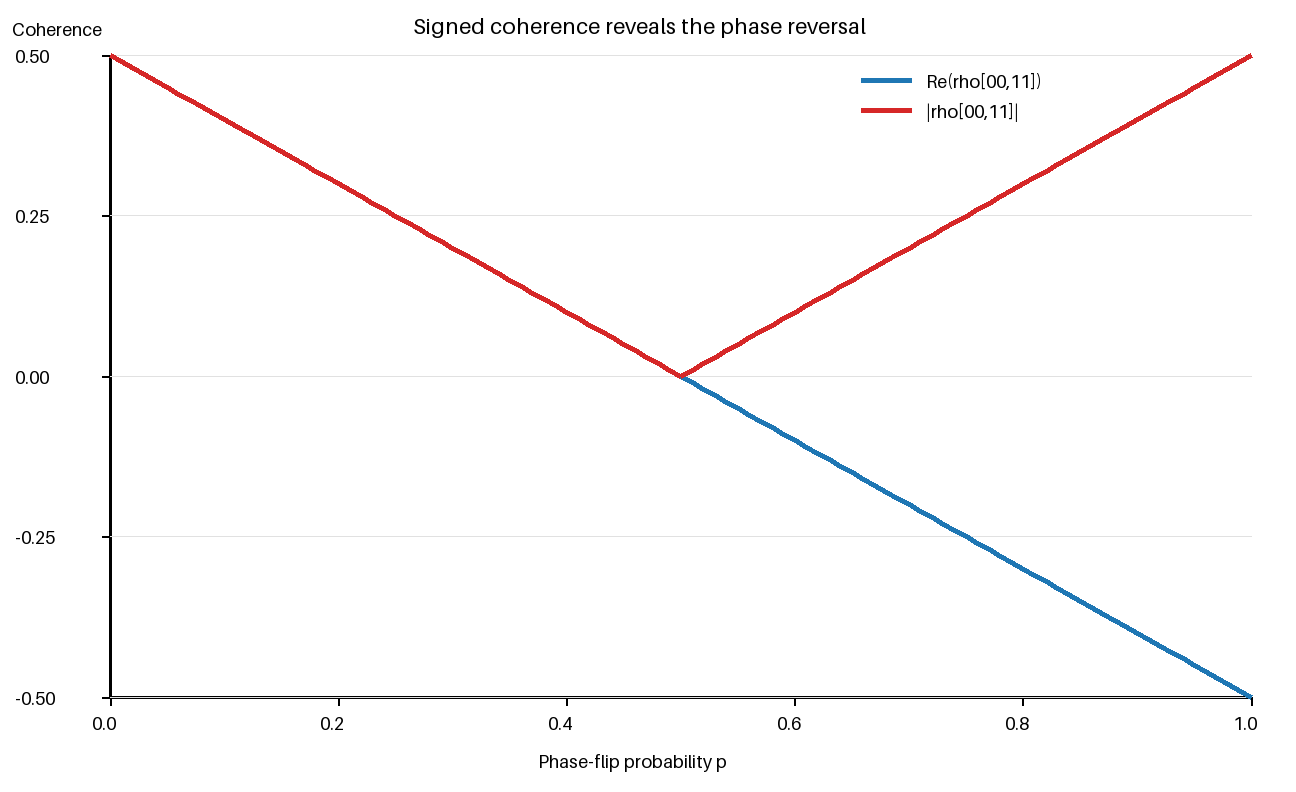
\includegraphics[width=0.86\linewidth]{coherence_real_vs_magnitude.png}
\caption{The real coherence crosses zero at $p=0.5$ and becomes negative,
whereas its magnitude returns to $0.5$.  At $p=1$ the state is the coherent
but orthogonal $|\Phi^-\rangle$, not the incoherent midpoint mixture.}
\label{fig:coherence}
\end{figure}

At $p=0.5$, the output is
\begin{equation}
\rho(0.5)=\tfrac12|00\rangle\langle00|+
\tfrac12|11\rangle\langle11|,
\end{equation}
which has no $|00\rangle\!\langle11|$ coherence but still has $S=1$.  At
$p=1$, $\rho(1)=|\Phi^-\rangle\langle\Phi^-|$: coherence magnitude is restored,
its sign is reversed, fidelity to $|\Phi^+\rangle$ is zero, and $S$ is still one.

\section{Conclusion}
Yes.  Computational-basis success probability alone can judge this noisy
Bell-state circuit as perfectly successful after its coherence has vanished or
its relative phase has reversed.  In this model $S(p)=1$ for all $p$, while
$F(p)=1-p$ and $\operatorname{Re}(\rho_{00,11})=(1-2p)/2$.  A benchmark intended
to certify Bell-state preparation must therefore include phase-sensitive
information rather than only the accepted computational-basis outcomes.

\section{Discussion}
This study is deliberately narrow.  It is an analytic density-matrix result
reproduced by deterministic classical simulation, not hardware data.  A
phase-flip channel is a simplified model, and no SPAM error, crosstalk,
coherent calibration error, finite-shot uncertainty, or drift is included.
The channel is applied after an ideal Bell circuit rather than assigned to a
specific pulse or time location inside a physical CNOT implementation.  The
results therefore do not estimate the CNOT error rate of an IBM device or any
other processor, and they do not constitute randomized benchmarking or full
CNOT characterization.

A second limitation is metric scope.  Fidelity to one target answers whether
the state matches $|\Phi^+\rangle$; it is not by itself a complete description
of a general quantum process.  Coherence magnitude likewise loses the sign
that distinguishes $|\Phi^+\rangle$ from $|\Phi^-\rangle$.  The comparison is
useful precisely because the metrics expose different projections of the same
state.

\bibliographystyle{plain}
\bibliography{references}
\end{document}

